\documentclass{../zkdl-presentation-template}

\title[Криптографія]{\textbf{Практичне №8. Геш-функції. Добування коренів за складеним модулем. Криптосистема Rabin}}

\date{18.11.2025}


\begin{document}
    \frame{
        \titlepage
    }
  
    \begin{frame}{Plan}
        \tableofcontents
    \end{frame}

\section{Геш-функції} % Note all sections and subsections are automatically placed in your table of contents

%------------------------------------------------
\begin{frame}{Означення}
            \begin{figure}
            \centering
            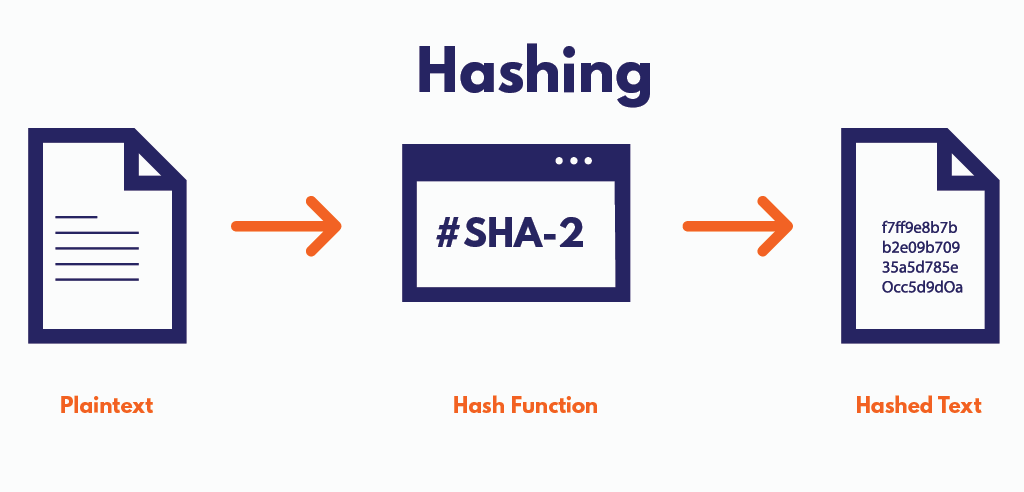
\includegraphics[width=0.8\linewidth]{8-crypto-practice/hash-function.png}
        \end{figure}
        \begin{definition}
            Геш-функцією в криптографії називають відображення:
            \begin{align*}
                h(X):\{0,1\}^*\rightarrow\{0,1\}^m, \quad m=\text{const},\quad m\in \mathbb{N} 
            \end{align*}
        \end{definition}
    \end{frame}
    
    \begin{frame}{Властивості геш-функцій}
        \begin{definition}
        \begin{enumerate}
            \item $\forall X\in \{0,1\}^*$ геш-значення $H=h(X)$ обчислюється швидко, тобто існує алгоритм поліноміальної часової складності від $n$.
            \item Геш-функція чутлива до будь-якої зміни вхідної послідовності. 
            \item Геш-функція має рівномірність виходів.
            \item $h(X)$ --- обчислювально одностороння функція, тобто для будь-якого $H\in \{0,1\}^m$ неможливо знайти хоча б одне $M$, таке що $H=h(M)$.
            \item Геш-функція має стійкість до колізій.
        \end{enumerate}
        \end{definition}
    \end{frame}

%------------------------------------------------
\begin{frame}
    \frametitle{1 Модель (Слабка Колізія)}
        \begin{figure}
            \centering
            
\includegraphics[width=1\linewidth]{2-crypto-sym/images/cells.png}
        \end{figure}
    
\end{frame}
%------------------------------------------------
\begin{frame}
    \frametitle{2 Модель (сильна колізія)}
    \begin{figure}
        \centering
        
\includegraphics[width=1\linewidth]{2-crypto-sym/images/cells.png}
    \end{figure}
\end{frame}
%------------------------------------------------
\begin{frame}
    \frametitle{3 Модель (атака Ювала)}
    \begin{figure}
        \centering
        
\includegraphics[width=1\linewidth]{2-crypto-sym/images/cells.png}
    \end{figure}
\end{frame}
%------------------------------------------------
\begin{frame}
    \frametitle{Атаки}
        \begin{block}{}
        \begin{itemize}
            \item Слабка колізія (пошук прообразу)
            \begin{align*}
                P_1=1-e^{-\frac{t}{2^m}}
            \end{align*}
            \item Сильна колізія (пошук другого прообразу або атака днів народжень)
            \begin{align*}
                P_2=1-e^{-\frac{t^2}{2^{m+1}}}
            \end{align*}
            \item Атака Ювала
            \begin{align*}
                P_3=1-e^{-\frac{t_1\cdot t_2}{2^{m}}}
            \end{align*}
        \end{itemize}

    	\end{block}
    
\end{frame}
\begin{frame}
    \frametitle{Задачі}
        \begin{block}{}
        Білет лотереї має номер з 5 десяткових цифр. Продано всі $100 000$ білетів. У розіграші вибираються випадковим чином $1000$ номерів (можуть повторюватись)
        \begin{itemize}
            \item з якою ймовірністю виграє той, хто купив один квиток?
            \item з якою ймовірністю виграє той, хто купив 1000 квитків?
            \item скільки білетів потрібно купити, щоб ймовірність виграшу була 0.5?
        \end{itemize}
    	\end{block}
        \begin{figure}
            \centering
            
\includegraphics[width=1\linewidth]{2-crypto-sym/images/cells_small.png}
        \end{figure}
    
\end{frame}
%------------------------------------------------
\section{Квадратичні лишки}
%------------------------------------------------
\begin{frame}
    \frametitle{Задачі}
        \begin{block}{}
        Нехай $p$ -- просте, $a\in Q_p$. Скільки квадратичних лишків та квадратичних нелишків буде міститись серед квадратних коренів $a$? Дати відповідь у випадку, коли $p=4k+3$.
        \begin{figure}
            \centering
            
\includegraphics[width=0.95\linewidth]{2-crypto-sym/images/cells.png}
        \end{figure}

    \end{block}
\end{frame}
%------------------------------------------------
\section{Корені квадратні за модулем}
%------------------------------------------------
%------------------------------------------------
\begin{frame}
    \frametitle{Добування за складеним модулем $n=pq$}
    Очевидно, що для добування кореня квадратного від числа $a$ за складеним модулем $n=pq$, число повинно бути квадратичним лишком як за $p$, так і за $q$. Якщо ці умови виконуються, то ми можемо обчислити наступні рівняння:
    \begin{gather*}
        x^2=a\text{ mod }p \qquad\qquad x^2=a\text{ mod }q
    \end{gather*}
    Кожне рівняння дає по два відповідні корені $\pm x_p, \pm x_q$. Тоді розв'язок початкового рівняння буде задовольняти наступній системі рівнянь:
    \begin{align*}
         \left\{ \begin{array}{r}
x=\pm x_p \text{ mod } p  \\ 
x=\pm x_q \text{ mod } q 
\end{array}\right.
    \end{align*}
    Розписавши цю систему як 4 системи і вирішивши кожну із них за Китайською теоремою про лишки, отримаємо \textbf{4 корені}.
    
\end{frame}
%------------------------------------------------
\begin{frame}
    \frametitle{Китайська теорема про лишки}
    \begin{block}{}
        Нехай

        \vspace{-9mm}
        \begin{align*}
            a_1,\dots, a_n\in\mathbb{N},\quad m_1,\dots,m_n:(m_i,m_j)=1,i\neq j,
        \end{align*}

        \vspace{-3mm}
        тоді існує єдиний розв'язок систем конгруенцій $x_0$ на інтервалі від 0 до $M-1$, де $M=m_1\cdot m_2\cdot\dots\cdot m_n:$

        \vspace{-6mm}
        \begin{align*}
                     \left\{ \begin{array}{r}
x\equiv a_1 \text{ mod } m_1  \\ 
x\equiv a_2 \text{ mod } m_2 \\ 
...\quad\quad\quad
\\
x\equiv a_n \text{ mod } m_n \\
\end{array}\right.
    \end{align*}
    Нехай 

    \vspace{-9mm}
    \begin{gather*}
        M_i=\frac{M}{m_i},\quad
        N_i=M_i^{-1}\mod m_i
    \end{gather*}
    тоді

    \vspace{-9mm}
    \begin{gather*}
        x_0=\sum_{i=1}^{n}a_iM_iN_i\mod M, \quad
        x=x_0+kM, k\in \mathbb{Z}.
    \end{gather*}
    \end{block}
\end{frame}
%-----------------------------------------------
\begin{frame}
    \frametitle{Універсальний метод 2:)}
    \begin{figure}
        \centering
        
\includegraphics[width=1\linewidth]{2-crypto-sym/images/cells.png}
        \label{fig:placeholder}
    \end{figure}
\end{frame}
%------------------------------------------------
\section{Протокол Rabin}
%------------------------------------------------
\begin{frame}
    \frametitle{Протокол}
        \begin{gather*}
            x^2\equiv a \text{ mod }n, \quad n=p\cdot q 
        \end{gather*}
            \begin{align*}
         \left\{ \begin{array}{r}
x^2= a \text{ mod } p, \left(\frac{a}{p}\right)=1  \\ 
x^2=a \text{ mod } q, \left(\frac{a}{q}\right)=1
\end{array}\right.
    \end{align*}
    \begin{columns}[c] % [c] вирівнювання по центру вертикалі
          \column{0.5\textwidth}
          \begin{align*}
\left\{ \begin{array}{r}
x=\pm \sqrt{a} \text{ mod } p  \\ 
x=\pm \sqrt{a} \text{ mod } q 
\end{array}\right.
\end{align*}
\column{0.5\textwidth}
\begin{align*}
\left\{ \begin{array}{r}
x=\pm x_p \text{ mod } p  \\ 
x=\pm x_q \text{ mod } q 
\end{array}\right.
\end{align*}
      \end{columns}
      \begin{figure}
          \centering
          
\includegraphics[width=1\linewidth]{2-crypto-sym/images/cells_small.png}
      \end{figure}
\end{frame}
%------------------------------------------------
\begin{frame}
    \frametitle{Задачі}
        \begin{block}{}
        Сформулюйте алгоритм розв’язання квадратичних порівнянь виду

        \vspace{-9mm}
        \begin{align*}
            ax^2+bx+c \equiv 0 \mod p
        \end{align*}

        \vspace{-5mm}
        де $p>2$ та $a \neq0 \mod p$.
            
\includegraphics[width=0.95\linewidth]{2-crypto-sym/images/cells.png}
    	\end{block}
\end{frame}
%------------------------------------------------
\begin{frame}
    \frametitle{Задачі}
        \begin{block}{}
         Нехай $p>2$ -- просте число i $x_0$ -- розв’язок порівняння \\$x^2\equiv a\mod p$.
Доведіть, що розв’язок порівняння \\$x^2\equiv a\mod p^2$ можна знайти у формі
$x=x_0+pt$ та покажіть, як його обчислювати.

\includegraphics[width=0.95\linewidth]{2-crypto-sym/images/cells.png}
    	\end{block}
\end{frame}
%-----------------------------------------------
\section{Криптоаналіз шифрів}
%-----------------------------------------------
\begin{frame}{Задачі}
    \begin{block}{}
        1. Покажіть, що функція RSA зберігає символ Якобі \\
        2. Покажіть, що при $e=\frac{\phi(n)}{2}+1$ функція RSA перетворюється на тотожню.
        
\includegraphics[width=1\linewidth]{2-crypto-sym/images/cells.png}
    \end{block}
\end{frame}

    \begin{frame}[plain, standout]
    \begin{figure}
        \centering
        
\includegraphics[width=0.9\linewidth]{Cryptocats.jpg}
        \label{fig:placeholder}
    \end{figure}
    \centering
    \LARGE
    \textbf{Питання?} \\

    \vspace{0.2cm} \Huge \ding{170} \large \\

  \end{frame}
\end{document}